%\documentclass{article}
%\usepackage{graphicx,subfigure}
%\begin{document}

\begin{figure}[!h]
  \centering
  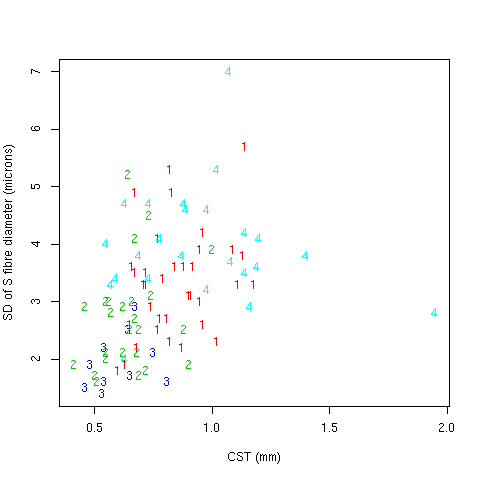
\includegraphics[width=1.0\textwidth]{cstdssd.png}
  \caption{Plot of CST measurements against standard deviation of secondary fibre diameter. The numbered points reveal the SkinType to which each data point belongs. The correlation of these points is 0.39 which is significant at the 1 percent level for 106 observations}
  \label{fig:cstdssd}
\end{figure}

%\end{document}

